%%% LaTeX Template: Article/Thesis/etc. with colored headings and special fonts
%%%
%%% Source: http://www.howtotex.com/

\documentclass[12pt]{article}


\usepackage{apuntes-estilo}
\usepackage{fancyhdr,lastpage}
\usepackage{color,colortbl}
\usepackage{verbatim}

\def\maketitle{

% Titulo 
 \makeatletter
 {\color{bl} \centering \huge \sc \textbf{
 Monitoreo de Recursos \\ 
\large \vspace*{-8pt} \color{black} Guía básica de Monitoreo de Recursos 
 \vspace*{8pt} }\par}
 \makeatother


% Autor
 \makeatletter
 {\centering \small 
 	Departamento de Ingeniería de Computadoras \\
 	Facultad de Informática - Universidad Nacional del Comahue \\
 	\vspace{20pt} }
 \makeatother

}

% Custom headers and footers
\fancyhf{} % clear all header and footer fields
\fancypagestyle{plain}{\fancyhf{}}
  	\pagestyle{fancy}
 	\lhead{\footnotesize Monitoreo de Recursos - Departamento de Ingeniería de Computadoras}
 	\rhead{\footnotesize \thepage\ }	% ''Page 1 of 2''

\def\ti#1#2{\texttt{#1} & #2 \\ }



\begin{document}

\thispagestyle{empty}
\maketitle
\setlength{\parindent}{0pt}

\section*{Introducción}

La administración de sistemas es mayormente un asunto de balancear los 
recursos disponibles con los usuarios y los programas que utilizan esos 
recursos. Por lo tanto, su carrera como administrador de sistemas será 
corta y completa de stress a menos que entienda completamente los recursos 
que tiene a su disposición.

Antes de poder supervisar recursos, primero tiene que conocer que recursos 
hay que monitorizar. En un apunte anterior hemos hablado de identificación 
de recursos. En general, todos los sistemas tienen disponibles los 
siguientes recursos:

\begin{itemize}
\item CPU
\item Memoria
\item Almacenamiento
\item Ancho de banda
\end{itemize}

Estos recursos tienen un impacto directo en el rendimiento del sistema y, 
por lo tanto, en la productividad y percepción de sus usuarios. Por ejemplo,
es clásico escuchar usuarios decir ``la computadora está lenta'', cuando 
en realidad lo que sucede es que el \textit{el ancho de banda} de
navegación por Internet no cumple las expectativas del usuario. 

En su aspecto más simple, monitorizar recursos no es más que obtener 
información concerniente a la utilización de uno o más recursos del sistema.
Sin embargo, esto raramente suele ser tan simple. Primero, debe tomar en 
cuenta los recursos a controlar. Luego es necesario examinar cada sistema 
a monitorizar, prestando especial atención a la situación de cada sistema.

Existen al menos dos objetivo por el cual es importante monitorizar un
sistema :

\begin{itemize}
\item El sistema está actualmente experimentando problemas de rendimiento
al menos parte del tiempo y a usted le gustaría mejorar su rendimiento. 
Comportamiento reactivo. 

\item El sistema está funcionando bien y le gustaría que se mantenga de esa 
manera. Comportamiento proactivo. 
\end{itemize}

La primera categoría indica que debería supervisar el sistema desde la 
perspectiva del rendimiento del sistema, mientras que la segunda categoría 
significa que debe supervisar los recursos del sistema desde la perspectiva
de planificación de la capacidad del mismo.

\section*{Monitorizar el rendimiento del sistema}

La supervisión del rendimiento del sistema se realiza normalmente como el 
primer y el último paso del siguiente proceso :

\begin{enumerate}
\item Monitorizar para identificar la naturaleza y ámbito de la escasez de 
recursos que están causando los problemas de rendimiento. 
\item Se analizan los datos producidos a partir de la supervisión y se toma
un curso de acción (normalmente optimización del rendimiento o la 
adquisición de hardware adicional)
\item Monitorizar para asegurarse de que se ha solucionado el problema de 
rendimiento. 
\end{enumerate}

 	
\fcolorbox{black}{grey}{
\parbox[t]{1.0\linewidth}{ \vspace*{0.4cm}
{\bf Lo importante:} 
Monitorizar el rendimiento del sistema a menudo es un proceso iterativo, 
repitiendo estos pasos varias veces para llegar al mejor rendimiento 
posible para el sistema. La razón principal para esto es que los recursos 
del sistema y su utilización tienden a estar estrechamente relacionados, 
lo que significa que a menudo la eliminación de un cuello de botella 
descubre otro más.
\vspace*{0.4cm} } }


\section*{¿Qué monitorizar?}

Los cuatro recursos básicos de un sistema a monitorizar son :

\begin{itemize}
\item CPU
\item Memoria
\item Almacenamiento
\item Ancho de Banda
\end{itemize}

Lamentablemente, no es tan simple. Por ejemplo, considere una unidad de 
disco. ¿Qué cosas podría querer saber sobre su utilización? Algunas posibles
preguntas: 

¿Cuánto espacio libre está disponible?

¿Cuántas operaciones de E/S (entrada/salida) realiza en promedio por
segundo?

¿Cuánto tiempo en promedio toma en completarse cada operación de E/S?

¿Cuántas de esas operaciones de E/S son lecturas? ¿Cuántas son escrituras?

¿Cuál es la cantidad promedio de datos leídos/escritos con cada E/S?

Hay más formas de estudiar el rendimiento de una unidad de disco; estos 
puntos solamente tocan la superficie. El concepto principal a tener en 
mente es que hay muchos tipos diferentes de datos para cada recurso.


\subsection*{¿Qué herramientas utilizar para monitorizar?}

Las herramientas básicas utilizadas para verificar los recursos son :
\begin{itemize}
\item free
\item top
\item vmstat
\item df y du 
\item La suite de herramientas de supervisión de recursos de 
\texttt{sysstat} (incluye iostat, sar, entre otros). 
\end{itemize}


\section*{Monitorizar la CPU}
En su forma más básica, monitorizar el poder de CPU significa determinar si
 la utilización de la CPU alcanza alguna vez el 100\%. Si la utilización 
de la CPU se mantiene por debajo de 100\%, sin importar lo que el sistema 
esté haciendo, hay poder de procesamiento adicional para más trabajo.

Sin embargo, es raro que un sistema no alcance el 100\% de utilización de 
CPU al menos una vez. En ese momento es importante examinar en más detalle 
los datos de utilización de CPU. Haciendo esto, se hace posible comenzar a 
determinar dónde se consume la mayoría del poder de procesamiento. A 
continuación mencionamos algunas de las estadísticas más populares de 
utilización de CPU.

Usuarios vs sistema: el porcentaje de tiempo consumido realizando 
procesamiento a nivel de usuario contra procesamiento a nivel de sistema, 
puede indicar si la carga de un sistema se debe principalmente a las 
aplicaciones que se están ejecutando o a la sobrecarga del sistema 
operativo. Altos porcentajes de procesamiento a nivel de usuario tiende a 
ser bueno (asumiendo que los usuarios están experimentando un rendimiento
satisfactorio), mientras que altos porcentajes de procesamiento a nivel de 
sistema tiende a apuntar hacia problemas que requerirían mayor 
investigación.

Procesos ejecutables: como vimos en el apunte anterior, un proceso puede 
tener diferentes estados. Por ejemplo, puede estar:
\begin{itemize}
\item Esperando porque se termine una operación de E/S.
\item Esperando porque el subsistema de administración de memoria 
resuelva un fallo de página.
\end{itemize}
En estos casos, el proceso no tiene necesidad de la CPU y se encuentra en
estado ``S, sleeping'' (durmiendo).  

Sin embargo, eventualmente el estado del proceso cambia y el proceso se 
vuelve ejecutable (``R, running''). Como su nombre lo implica, un proceso 
ejecutable es aquel capaz de realizar el trabajo tan pronto como reciba 
tiempo de CPU. Sin embargo, si hay más de un proceso ejecutable en un 
momento determinado, todos excepto uno de los procesos deben esperar por su 
turno de CPU (asumiendo que tenemos un solo CPU). Monitorizando el
número de procesos ejecutables, es posible determinar cuan comprometido 
está cada CPU en su sistema.

Otras métricas de rendimiento que reflejan un impacto en la utilización 
de la CPU tienden a incluir servicios diferentes que el sistema operativo 
proporciona a los procesos. Estas pueden incluir estadísticas sobre la 
administración de memoria, procesamiento de E/S, etc. Estas estadísticas 
también revelan que, cuando el rendimiento del sistema está siendo 
supervisado, no hay límites entre las diferentes estadísticas. En otras 
palabras, las estadísticas de utilización de CPU pueden terminar apuntando 
a un problema en el subsistema de E/S, o las estadísticas de utilización 
de memoria pueden revelar un defecto de una aplicación.

Por lo tanto, cuando esté supervisando el funcionamiento del sistema, no 
es posible examinar una estadística de forma totalmente aislada; solamente
mediante el examen del cuadro completo es posible extraer información 
significativa de cualquier estadística de rendimiento que reúna.

\subsection*{Ejemplo de monitoreo de la CPU}

El programa mas interesante para iniciar el monitoreo del sistema, y en 
particular de la CPU, es \textbf{top}.

\fcolorbox{black}{grey}{
\parbox[t]{1.0\linewidth}{ \vspace*{0.4cm}
{\bf top} proporciona una visión continuada de la actividad del procesador 
en tiempo real. Muestra un listado de las tareas  que  hacen  un  uso  
más intensivo  de  la  CPU en el sistema, y puede proporcionar una 
interfaz interactiva para manipular procesos. Puede clasificar  las  
tareas  por empleo  de CPU,  uso  de  memoria  y  tiempo  de  ejecución.
\vspace*{0.4cm} } }

\begin{center}
 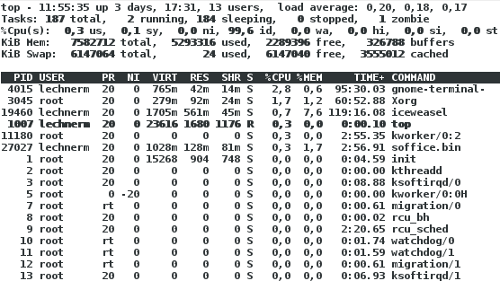
\includegraphics{top.png}
\end{center}

\subsubsection*{Descripciones de algunos campos de top}
\texttt{top} despliega  una variada información sobre el estado del 
procesador. La pantalla se actualiza cada tres segundos de forma 
predeterminada, pero esto se puede cambiar con la opción en la línea de 
comandos ``d'' o la orden interactiva ``d'' o ``s''.

Top muestra una sección de resumen, un encabezado con la enumeración de
campos por tarea y luego un listado de tareas. Dentro de la sección de
resumen encontramos la siguiente información:  

\begin{itemize}
\item \texttt{uptime}: la primer línea muestra el tiempo
 que el sistema ha  estado  activo,  y  las  tres medias de carga para el 
sistema. Las medias de carga son  el número medio de procesos listos  para
ejecutarse  o en estado durmiendo ininterrumpible, durante  los  últimos
1,  5  y  15  minutos.  La línea coincide con la salida del comando 
\texttt{uptime} y puede quitarse o agregarse con la orden interactiva 
``l'' (ele minúscula).
\item  Tasks: el  número  total  de  procesos ejecutándose durante  la  
última actualización. Este número también  se  divide  en  el  número 
de  tareas  que  están  ejecutándose, durmiendo, paradas o no-muertas 
(zombie).  Las líneas de procesos y estados pueden quitarse o ponerse con 
la orden interactiva ``t''.
\item  \%CPU: muestra el porcentaje de tiempo de CPU en modo de usuario 
(us), en modo  de sistema (sy), en tareas con la prioridad alterada por
 nice (ni) (ver página del manual para el comando \texttt{nice}), y el 
 tiempo  de  inactividad (id).  Las tareas con la prioridad alterada por 
nice son solamente aquéllas cuyo  valor  nice  es  negativo. El tiempo  
transcurrido  en  las tareas con la prioridad alterada por nice también 
se contará en el tiempo de sistema y de usuario,  así que  el  total  
será  superior  al  100\%. Las líneas de procesos y estados y tiempos
 de CPU pueden quitarse o agregarse  con  la  orden interactiva ``t''.
Si estamos en un sistema con más de una CPU, la orden interactiva ``1'' 
uno, desglosa la misma información por cada una de las CPU del sistema.
\item Mem: datos sobre el empleo de memoria principal, incluyendo la 
memoria disponible en total,  la  memoria  libre,  la  usada, y  la
utilizada  para  búferes.  La  línea  de la información de memoria puede 
agregarse o quitarse con la orden interactiva ``m''.
\item Swap: datos sobre el  espacio  de  intercambio,  incluyendo  el  
total,  el utilizado, el disponible  y  el ``cached''. Esto y Mem son 
sencillamente como la salida del comando \texttt{free}.
\end{itemize}

De manera predeterminada, en la sección de encabezado y tareas encontramos
la siguiente información (puede ampliarse o modificarse a conveniencia del
administrador, vea ``\texttt{man top}''):

\begin{itemize}
\item PID: auto-descriptivo. 
\item USER: usuario dueño de la tarea.
\item PR: indica la prioridad con la que se ejecuta el proceso. 
\item NI: valor ``nice'', un valor negativo indica mayor prioridad mientras
que un valor positivo indica menor prioridad. Un valor de cero significa
que la prioridad no será ajustada basada en este campo. 
\item VIRT: indica el monto total de memoria virtual (principal mas espacio
de intercambio) utilizada por el proceso. Incluye su código, datos y 
bibliotecas compartidas con otros procesos.  
\item RES: Se muestra aquí la cantidad total de memoria principal (física)
 utilizada  por el proceso.  
\item SHR: indica cantidad  de  memoria potencialmente compartida con otros
procesos.
\item S: indica el estado  de  la tarea. El estado puede ser S para 
durmiente, D para sueño no interrumpible, R para ejecución, Z para zombies,
o  T para detenidos o trazados (ver apunte anterior sobre Procesos). 
\item \%CPU La  porción  del  tiempo  de  CPU  consumido por la tarea desde
la última actualización de la pantalla, expresada como un  porcentaje del 
tiempo de CPU total. De manera predeterminada el valor mostrado no esta
normalizado por el número total de CPUs, esto es conocido como 
``modo Irix''. Si necesitamos el valor normalizado por la cantidad de CPUs,
es decir que se divida el porcentaje por el número de CPUs presentes, 
entonces requerimos lo que se conoce como ``modo Solaris''. Puede alternarse
entre modo Irix o Solaris mediante la orden interactiva ``I''. 
\item TIME+: indica el tiempo total de CPU que la tarea ha usado desde que 
empezó. Si el  modo  acumulativo está activado, también incluye el tiempo
de  CPU empleado por los hijos del proceso que hayan muerto. Uno puede
establecer  el  modo  acumulativo  con la orden interactiva  S.  
\item \%MEM: indica el porcentaje de la memoria física ocupada por la tarea.
\end{itemize}

\fcolorbox{black}{grey}{
\parbox[t]{1.0\linewidth}{ \vspace*{0.4cm}
{\bf top} la orden interactiva ``h'' presenta ayuda básica acerca de cómo
manipular la salida de top, campos mostrados, colores, etc. Recuerde mirar
la página del manual de top para hacer una correcta interpretación de los 
campos mostrados. 
\vspace*{0.4cm} } }

Los campos más utilizados para analizar la CPU son los que indican los 
porcentajes de \textbf{utilizado}, y de \textbf{ocioso}. Si los campos 
user+system están cercanos al 100\% puede indicar una falta de recurso de 
CPU, o bien que hay un proceso descontrolado. Como se dijo anteriormente, 
el análisis debe ser comprensivo, no aislado. 

La sección de procesos de top puede ser ordenada según diferentes campos, 
de manera predeterminada se ordena por \%CPU, de mayor a menor. Este 
ordenamiento nos permite observar los procesos que están consumiendo mayor
cantidad de procesamiento en el último intervalo de tiempo (vea la página
del manual de top para otros ordenamientos). 

\section*{Monitorizar el almacenamiento}
El monitoreo del almacenamiento normalmente tiene lugar en dos niveles 
diferentes:

\begin{itemize}
\item Monitorizar insuficiente espacio en disco.
\item Monitorizar problemas de rendimiento relacionados con el 
almacenamiento.
\end{itemize}

La razón de esto es que es posible tener problemas calamitosos en un área 
y ningún problema en otra. Por ejemplo, es posible causar que a la unidad 
de disco se le acabe el espacio sin causar ningún tipo de problemas 
relacionados al rendimiento. De la misma manera, es posible tener una 
unidad de disco que tiene 99\% de espacio libre, pero que se ha puesto más 
allá de sus límites en términos de rendimiento.

Sin embargo, es más probable que el sistema promedio experimente diferentes
 grados de escasez de recursos en ambas áreas. Debido a esto, es probable
 que — hasta cierto punto — los problemas en un área impacten a la otra. 
La mayoría de las veces este tipo de interacción toma la forma de 
funcionamientos de E/S más y más pobres cuando el sistema se acerca al
 0\% de espacio libre, en casos de cargas de E/S extremas, es posible 
reducir las salidas de E/S a tal nivel que las aplicaciones no se ejecutan 
adecuadamente.

En cualquier caso, las estadísticas siguientes son útiles para supervisar 
el almacenamiento:

\begin{itemize}
\item Espacio libre: es probablemente el recurso que todos los 
administradores de sistemas vigilan más de cerca; sería raro el 
administrador que no verifica el espacio disponible (o que tiene una 
forma de hacerlo automáticamente).

\item Estadísticas relacionadas al sistema de archivos: estas estadísticas
 (tales como el número de archivos/directorios, tamaño promedio de los 
archivos, etc.) suministran detalles adicionales sobre un porcentaje de 
espacio libre. Como tal, estas estadísticas hacen posible para los 
administradores de sistemas configurar el sistema para que entregue el 
mejor rendimiento, pues la carga de E/S impuesta por un sistema de 
archivos lleno de muchos pequeños archivos no es la misma que la carga 
impuesta por un sistema de archivos lleno con un único archivo enorme.

\item Transferencias por segundo: esta estadística es una buena forma de 
determinar si se están alcanzando las limitaciones de ancho de banda de 
un dispositivo en particular.

\item Lecturas/escrituras por segundo: con un desglose más detallado de 
las transferencias por segundo, estas estadísticas permiten al 
administrador de sistemas entender mejor la naturaleza de las cargas de 
E/S que está experimentando un dispositivo de almacenamiento. Esto puede 
ser crítico, ya que algunas tecnologías de almacenamiento tienen 
características de funcionamiento muy diferentes para operaciones de 
lecturas contra escrituras.
\end{itemize}

Los comandos \texttt{df} y \texttt{du} son útiles a la hora de encontrar 
estadísticas y mediciones sobre la utilización de sistemas de archivos 
montados. El primero obtiene porcentajes de utilización de los sistemas 
de archivos montados mientras que el segundo du  informa  de  la cantidad 
de espacio de disco usada por los archivos especificados, y por cada 
directorio en  las  jerarquías  cuyas  raíces estén  en  los  archivos 
especificados.  Aquí, ``espacio de disco usado'' significa espacio usado 
por la jerarquía de  ficheros  por  debajo  del fichero especificado. 

De este modo una secuencia clásica de uso de {\tt df} y {\tt du}, ante
una alarma disparada por falta de espacio en un sistema de archivos, será:

\begin{center}
 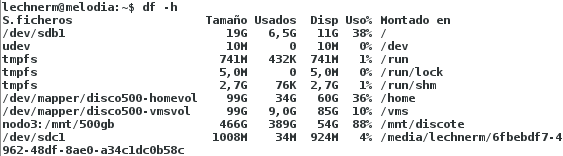
\includegraphics{df.png}
\end{center}

Es importante tener en cuenta que un porcentaje de uso puede ser o no
alarmante dependiendo del tamaño total. No es lo mismo un 90\% de uso en 
un sistema de archivos cuyo tamaño disponible es de 1000Gb, a un 90\% en 
uno de 10Gb. Los valores críticos serán definidos para cada file system 
considerando su uso y tasa estimada de crecimiento. 

Ahora bien, supongamos que el sistema de archivos a evaluar de la salida 
anterior es {\tt /home} (si bien en este momento no se encuentra bajo 
un límite crítico de uso)  y queremos saber cuáles son los directorios 
que consumen mas espacio en disco para este sistema de archivos, entonces
podemos averiguarlo haciendo: 

\begin{center}
 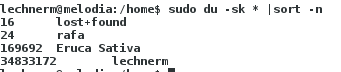
\includegraphics{du.png}
\end{center}

El comando {\tt du -sk |sort -n} indica a du realizar la suma (-s) de todos
los archivos contenidos en el directorio, y devolver el valor en kilo bytes
(-k). La salida se la enviamos al comando {sort} que ordena numéricamente 
(-n) lo recibido por du. De este modo, en la parte inferior de la salida 
vemos los archivos y directorios que consumen mas espacio dentro del 
directorio home. 

\section*{Monitorizar la memoria}
Si existe un área en la que se puede encontrar gran cantidad de 
estadísticas de rendimiento, esta área es la utilización de la memoria. 
Debido a la complejidad inherente de los sistemas operativos con memoria 
virtual bajo demanda de hoy día, las estadísticas de utilización de memoria
 son muchas y variadas. 

\subsection*{Ejemplo de monitoreo de la memoria}

Usando el comando \texttt{free} es posible obtener una vista general 
concisa (quizás hasta un poco simplista) de la utilización de la memoria
principal y de intercambio. He aquí un ejemplo:

\begin{center}
 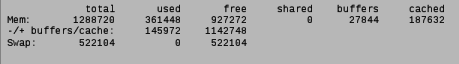
\includegraphics{free1.png}
\end{center}

Podemos ver que este sistema tiene 1.2GB de RAM, de los que solamente 
350MB están realmente en uso. Como se puede esperar para un sistema con 
esta cantidad de RAM disponible, no se utiliza nada de los 500MB de 
memoria de intercambio.

Compare ese ejemplo con el que sigue:

\begin{center}
 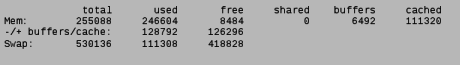
\includegraphics{free2.png}
\end{center}

      
Este sistema tiene alrededor de 256MB de RAM, la mayoría de la cual está 
en uso, dejando solamente 8MB libres. Más de 100MB de los 512MB de swap 
están en uso. Aún cuando el sistema está ciertamente más limitado en 
términos de memoria que el primer sistema, para determinar si esta 
limitación de memoria está causando problemas de rendimiento, tenemos 
que investigar un poco más.

El comando \texttt{vmstat} reporta estadísticas acerca del uso de la memoria
virtual del sistema. Aún cuando su salida es más críptica que free, tiene 
el beneficio mostrar más que simplemente las estadísticas de utilización de
memoria. He aquí la salida de ``\texttt{vmstat 1 10}'':

\begin{center}
 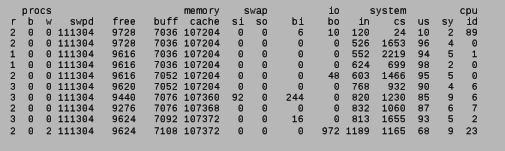
\includegraphics{vmstat2.png}
\end{center}

Durante esta muestra de 10 capturas de 1 segundos de duración cada una, la 
cantidad de memoria libre (el campo free) varía de alguna forma, y hay un poco de E/S relacionada con la memoria de intercambio (los campos si y so), pero en general, este sistema está funcionando bien. 

La primera línea de vmstat reporta las estadísticas desde el último reinicio
de sistema. Mientras que las restantes líneas serán las estadísticas de 
períodos de 1 segundo. 

Las columnas bajo ``procs'' dan información sobre estado de los procesos.
Las columnas bajo ``memory'' se refieren a memoria principal (física), las
columnas bajo ``swap'' se refieren a estadísticas relacionadas al espacio 
de intercambio, las columnas bi/bo bajo io se refieren a estadísticas de 
bloques por segundos enviados o recibidos desde los discos, las columnas
bajo ``system'' se refieren a estadísticas relacionadas a interrupciones y
cambios de contexto, y finalmente las columnas bajo ``cpu'' indican 
estadísticas de cómo se está utilizando el tiempo de cpu (sistema, usuario, 
ocioso, etc). Para más información consulte la página de manual de vmstat. 

La supervisión exitosa de la utilización de la memoria requiere una buena 
comprensión de cómo funciona la memoria virtual bajo demanda de un sistema 
operativo.

{\bf Identificando culpables}

Volviendo al comando \texttt{top}, podemos ordenar la salida por VIRT o RES
para analizar cuáles son los procesos que actualmente se encuentran 
consumiendo mayor cantidad de memoria: 

\begin{center}
 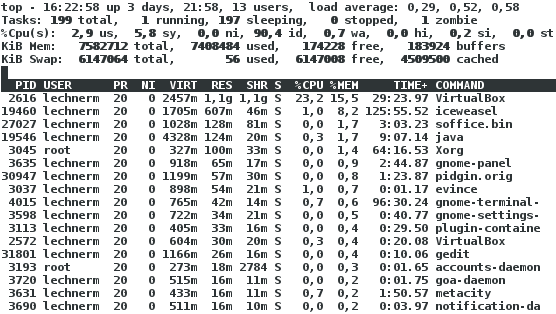
\includegraphics{topmem.png}
\end{center}

Este análisis complementa lo anteriormente visto con free y vmstat a la
hora de encontrar responsables ante un posible comportamiento anormal 
de los procesos en ejecución, o bien para un simple análisis que pueda 
disparar una posible una posible actualización de recursos del sistema. 

\section*{Monitorizar el ancho de banda}
Monitorizar el ancho de banda es más complicado que la supervisión de otros recursos descritos aquí. La razón de esto se debe al hecho de que las estadísticas de rendimiento tienden a estar basadas en dispositivos, mientras que la mayoría de los lugares en los que es importante el ancho de banda tienden a ser los buses que conectan dispositivos. En lo casos donde más de un dispositivo comparte un bus común, puede encontrar estadísticas razonables para cada dispositivo, pero la carga que esos dispositivos colocan en el bus es mucho mayor.

Otro reto al monitorizar el ancho de banda es que pueden existir circunstancias donde las estadísticas para los dispositivos mismos no estén disponibles. Esto es particularmente verdadero para los buses de expansión del sistema y datapaths[2]. Sin embargo, aún cuando no siempre tendrá disponibles estadísticas relacionadas al ancho de banda 100\% exactas, a menudo se encuentra información suficiente para hacer posible cierto nivel de análisis, particularmente cuando se toman en cuenta estadísticas relacionadas.

\subsection*{Ejemplo de monitoreo del ancho de banda}

Usando vmstat, es posible determinar si es excesiva la actividad general de los dispositivos examinando los campos bi y bo; además, revisando los campos si y so le dará un poco más de conocimiento sobre cuánta actividad de disco se debe a E/S relacionada a swap.

\begin{center}
 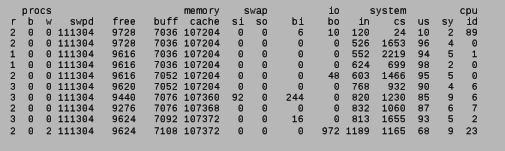
\includegraphics{vmstat2.png}
\end{center}

        
En este ejemplo, el campo bi muestra dos bloques/segundos escritos a los dispositivos en bloque (principalmente unidades de disco), mientras que el campo bo muestra seis bloques/segundos leído desde los dispositivos de bloque. Podemos determinar que ninguna de esta actividad se debe a intercambio de memoria (swap), ya que los campos si y so ambos muestran una tasa de E/S relacionada a swap de cero kilo bytes/segundo.

Usando iostat, es posible obtener un poco más de detalles sobre la actividad relacionada al disco:

\begin{center}
 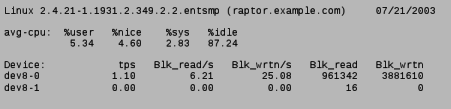
\includegraphics{iostat1.png}
\end{center}

Esta salida nos muestra que el dispositivo con un número major de 8 (el cual es /dev/sda, el primer disco SCSI) tiene un promedio un poco mayor de una operación de E/S por segundo (el campo tsp). La mayoría de la actividad de E/S para este dispositivo fueron escrituras (el campo Blk\_wrtn), con un poco más de 25 bloques escritos cada segundo (el campo Blk\_wrtn/s).

Si se necesitan más detalles, utilice la opción -x de iostat:

\begin{center}
 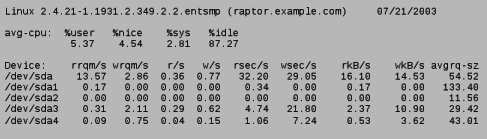
\includegraphics{iostat2.png}
\end{center}

        
Más allá de las largas líneas conteniendo más campos, la primera cosa a tener en mente es que esta salida de iostat está mostrando ahora estadísticas a un nivel de partición. Usando df para asociar los puntos de montaje con los nombres de dispositivos, es posible utilizar este informe para determinar si, por ejemplo, la partición conteniendo /home/ está experimentando una sobrecarga excesiva.

En realidad, cada línea de salida de iostat -x es más larga y contiene más información que esto; he aquí el resto de cada línea (agregando la columna del dispositivo para facilitar la lectura):

\begin{center}
 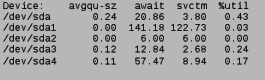
\includegraphics{iostat3.png}
\end{center}

        
En este ejemplo, es interesante observar que /dev/sda2 es la partición swap del sistema; obviamente, a partir de los muchos campos de esta partición que leen 0.00, el swapping no es un problema en el sistema.

Otro punto interesante a tomar en cuenta es /dev/sda1. Las estadísticas para esta partición son inusuales; la actividad general parece baja, pero por qué el tamaño promedio de peticiones de E/S (el campo avgrq-sz), el tiempo promedio de espera (el campo await) y el tiempo promedio de servicio (el campo svctm) son mucho más grandes que en las otras particiones? La respuesta es que esta partición contiene el directorio /boot/, el cual es donde el kernel y el disco inicial ramdisk son almacenados. Cuando el sistema arranca, las lecturas de E/S (observe que solamente los campos rsec/s y rkB/s son diferentes de cero; no se hace ninguna escritura aquí de forma regular) usadas durante el proceso de arranque son para grandes números de bloques, resultando en despliegues iostat de esperas relativamente largas y tiempos de servicios.








\section*{Licencia}

Este texto es una modificación del texto original 
''Red Hat Enterprise Linux 4
Introducción a la administración de sistemas'', realizada por Red Hat.

Documento original: 
\begin{verbatim}
http://web.mit.edu/rhel-doc/4/RH-DOCS/rhel-isa-es-4/index.html
\end{verbatim}

Licencia de la documentación original: 
Copyright © 2005 por Red Hat, Inc. Este material solamente se distribuye bajo los términos y condiciones establecidas en la Open Publication License, V1.0 o versiones posteriores (la última versión está disponible en http://www.opencontent.org/openpub/).

Esta versión modificada fue realizada por Rafael Ignacio Zurita para el curso ''Administración de Sistemas'' de la carrera
''Tecnicatura Universitaria en Administración de Sistemas y Software Libre''. Se mantiene la licencia original.

\end{document}
